% Practice Test 11 — Alaska Edition
% Questions: 30 (19 MC + 11 SA)
% Generated by scripts/generate_practice_tests.py

\begin{practiceQuestion}{1-3-q09}{mc}
\begin{questionText}
Find $k$ from the table.

\begin{center}
\begin{tabular}{|c|c|}
\hline $x$ & $y$ \\ \hline $6$ & $9$ \\ $10$ & $15$ \\ $14$ & $21$ \\ \hline
\end{tabular}
\end{center}
\end{questionText}
\choiceA{$1.5$}
\choiceB{$3$}
\choiceC{$\frac{2}{3}$}
\choiceD{$6$}
\correctAnswer{A}
\explanation{$k = \frac{9}{6} = 1.5$. Check: $\frac{15}{10} = 1.5$ and $\frac{21}{14} = 1.5$.}
\end{practiceQuestion}

\begin{practiceQuestion}{1-5-q11}{mc}
\begin{questionText}
A proportional graph passes through $(5, 12.5)$. What is the equation of this line?
\end{questionText}
\choiceA{$y = 5x$}
\choiceB{$y = 2.5x$}
\choiceC{$y = 12.5x$}
\choiceD{$y = 7.5x$}
\correctAnswer{B}
\explanation{$k = \frac{12.5}{5} = 2.5$, so the equation is $y = 2.5x$.}
\end{practiceQuestion}

\begin{practiceQuestion}{1-6-q13}{mc}
\begin{questionText}
An architect's model uses a scale of $1$ inch $= 3$ feet. If a room in the model is $5.5$ inches long, what is the actual length?
\end{questionText}
\choiceA{$8.5$ feet}
\choiceB{$15$ feet}
\choiceC{$16.5$ feet}
\choiceD{$18$ feet}
\correctAnswer{C}
\explanation{Actual length $= 5.5 \times 3 = 16.5$ feet.}
\end{practiceQuestion}

\begin{practiceQuestion}{2-2-q08}{mc}
\begin{questionText}
$15$ is what percent of $125$?
\end{questionText}
\choiceA{$10\%$}
\choiceB{$12\%$}
\choiceC{$15\%$}
\choiceD{$18\%$}
\correctAnswer{B}
\explanation{$\frac{15}{125} = \frac{p}{100}$. Cross-multiply: $125p = 1500$. Divide: $p = 12\%$.}
\end{practiceQuestion}

\begin{practiceQuestion}{2-5-q03}{mc}
\begin{questionText}
A concert ticket costs $\$65$. There is a $15\%$ service fee. What is the total?
\end{questionText}
\choiceA{$\$9.75$}
\choiceB{$\$55.25$}
\choiceC{$\$74.75$}
\choiceD{$\$80.00$}
\correctAnswer{C}
\explanation{$65 \times 1.15 = \$74.75$.}
\end{practiceQuestion}

\begin{practiceQuestion}{3-1-q09}{mc}
\begin{questionText}
Which integer is its own opposite?
\end{questionText}
\choiceA{$1$}
\choiceB{$-1$}
\choiceC{$0$}
\choiceD{No integer is its own opposite}
\correctAnswer{C}
\explanation{The opposite of $0$ is $0$ because $0 + 0 = 0$. Zero is the only integer that is its own opposite.}
\end{practiceQuestion}

\begin{practiceQuestion}{3-2-q09}{mc}
\begin{questionText}
A diver is at $-20$ feet. She rises $8$ feet. What is her new depth?
\end{questionText}
\choiceA{$-28$ feet}
\choiceB{$-12$ feet}
\choiceC{$12$ feet}
\choiceD{$28$ feet}
\correctAnswer{B}
\explanation{$(-20) + 8 = -12$. Rising from a negative position adds a positive: $20 - 8 = 12$, keep negative.}
\end{practiceQuestion}

\begin{practiceQuestion}{3-3-q08}{mc}
\begin{questionText}
What is the distance between $-9$ and $4$ on a number line?
\end{questionText}
\choiceA{$5$ units}
\choiceB{$-5$ units}
\choiceC{$13$ units}
\choiceD{$-13$ units}
\correctAnswer{C}
\explanation{Distance $= |{-9} - 4| = |{-13}| = 13$ units. Distance is always positive.}
\end{practiceQuestion}

\begin{practiceQuestion}{3-10-q27}{gmc}
\begin{questionText}
The elevation diagram shows three locations.

\begin{center}
\begin{tikzpicture}[scale=0.4]
  \draw[thick,->] (0,-6) -- (0,8);
  \foreach \y in {-5,...,7} \draw (-0.3,\y) -- (0.3,\y);
  \node[right=6pt] at (0,5) {$500$ ft};
  \node[right=6pt] at (0,0) {Sea Level};
  \node[right=6pt] at (0,-4) {$-400$ ft};
  \fill[funBlue] (0,6) circle (5pt) node[left=10pt] {Peak: $600$ ft};
  \fill[funGreen] (0,1) circle (5pt) node[left=10pt] {Town: $100$ ft};
  \fill[funRed] (0,-3) circle (5pt) node[left=10pt] {Mine: $-300$ ft};
  \draw[dashed,gray] (-0.5,0) -- (0.5,0);
\end{tikzpicture}
\end{center}

What is the distance from the mine to the peak?
\end{questionText}
\choiceA{$300$ ft}
\choiceB{$600$ ft}
\choiceC{$900$ ft}
\choiceD{$-900$ ft}
\correctAnswer{C}
\explanation{$600 - (-300) = 600 + 300 = 900$ ft.}
\end{practiceQuestion}

\begin{practiceQuestion}{4-1-q30}{gsa}
\begin{questionText}
The diagram shows a rectangle with the dimensions shown.

\begin{center}
\begin{tikzpicture}[scale=0.8]
  \draw[thick, fill=funBlue!10] (0,0) rectangle (5,3);
  \node[above] at (2.5,3) {$3x + 2$};
  \node[right] at (5,1.5) {$4$};
\end{tikzpicture}
\end{center}

Write an expression for the area of the rectangle, then evaluate it when $x = 3$.
\end{questionText}
\correctAnswer{$12x + 8$; $44$ square units}
\explanation{Area $=$ length $\times$ width $= 4(3x + 2) = 12x + 8$. When $x = 3$: $12(3) + 8 = 36 + 8 = 44$ square units.}
\end{practiceQuestion}

\begin{practiceQuestion}{5-2-q22}{sa}
\begin{questionText}
A ride-share app charges $\$2.50$ per mile plus a $\$3.00$ base fee. The total fare was $\$15.50$. How many miles was the ride?
\end{questionText}
\correctAnswer{$5$ miles}
\explanation{$2.50m + 3 = 15.50$. Subtract $3$: $2.50m = 12.50$. Divide by $2.50$: $m = 5$.}
\end{practiceQuestion}

\begin{practiceQuestion}{5-3-q16}{mc}
\begin{questionText}
Solve $8(x + 1) = 48$.
\end{questionText}
\choiceA{$x = 5$}
\choiceB{$x = 6$}
\choiceC{$x = 7$}
\choiceD{$x = \dfrac{47}{8}$}
\correctAnswer{A}
\explanation{Divide by $8$: $x + 1 = 6$. Subtract $1$: $x = 5$. Check: $8(5 + 1) = 8(6) = 48$ \checkmark.}
\end{practiceQuestion}

\begin{practiceQuestion}{5-4-q04}{mc}
\begin{questionText}
Which is the best first step to solve $\dfrac{x}{4} + \dfrac{1}{2} = 3$?
\end{questionText}
\choiceA{Subtract $\frac{1}{2}$ from both sides}
\choiceB{Multiply every term by $4$}
\choiceC{Divide both sides by $4$}
\choiceD{Add $\frac{1}{2}$ to both sides}
\correctAnswer{B}
\explanation{Multiplying every term by $4$ (the LCD) clears the fractions: $x + 2 = 12$.}
\end{practiceQuestion}

\begin{practiceQuestion}{5-5-q14}{mc}
\begin{questionText}
Solve $7 - 2x < 1$.
\end{questionText}
\choiceA{$x < 3$}
\choiceB{$x > 3$}
\choiceC{$x < -3$}
\choiceD{$x > -3$}
\correctAnswer{B}
\explanation{Subtract $7$: $-2x < -6$. Divide by $-2$ and flip: $x > 3$.}
\end{practiceQuestion}

\begin{practiceQuestion}{5-6-q20}{sa}
\begin{questionText}
Solve $-5x + 15 \geq 30$. Describe the graph.
\end{questionText}
\correctAnswer{$x \leq -3$; closed circle at $-3$, shade left}
\explanation{Subtract $15$: $-5x \geq 15$. Divide by $-5$ and flip: $x \leq -3$. Closed circle at $-3$, shade left.}
\end{practiceQuestion}

\begin{practiceQuestion}{6-2-q26}{gmc}
\begin{questionText}
The original drawing below uses scale $1$ cm $= 10$ m. You are asked to redraw the rectangle at scale $1$ cm $= 5$ m. What will the new dimensions be?

\begin{center}
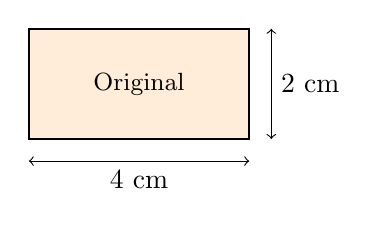
\begin{tikzpicture}[scale=0.7]
  \draw[thick,fill=orange!15] (0,0) rectangle (4,2);
  \draw[<->] (0,-0.4) -- (4,-0.4);
  \node[below] at (2,-0.4) {$4$ cm};
  \draw[<->] (4.4,0) -- (4.4,2);
  \node[right] at (4.4,1) {$2$ cm};
  \node at (2,1) {\small Original};
\end{tikzpicture}
\end{center}
\end{questionText}
\choiceA{$2$ cm by $1$ cm}
\choiceB{$4$ cm by $2$ cm}
\choiceC{$8$ cm by $4$ cm}
\choiceD{$20$ cm by $10$ cm}
\correctAnswer{C}
\explanation{Scale ratio: $\frac{10}{5} = 2$. New dimensions: $4 \times 2 = 8$ cm by $2 \times 2 = 4$ cm.}
\end{practiceQuestion}

\begin{practiceQuestion}{6-3-q29}{gsa}
\begin{questionText}
Look at the triangle below. Two angles are given. Can this triangle exist? If so, what is the third angle?

\begin{center}
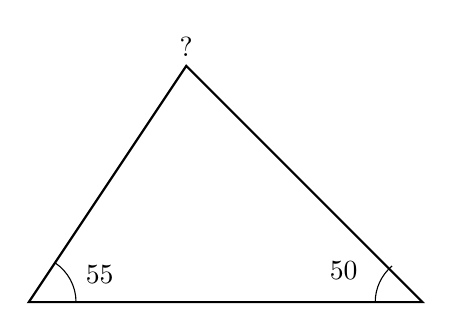
\begin{tikzpicture}[scale=1]
  \draw[thick] (0,0) -- (5,0) -- (2,3) -- cycle;
  \draw (0.6,0) arc[start angle=0,end angle=56,radius=0.6];
  \node at (0.9,0.35) {$55°$};
  \draw (4.4,0) arc[start angle=180,end angle=130,radius=0.6];
  \node at (4,0.4) {$50°$};
  \node[above] at (2,3) {$?$};
\end{tikzpicture}
\end{center}
\end{questionText}
\correctAnswer{Yes; the third angle is $75°$}
\explanation{$180° - 55° - 50° = 75°$. The angles sum to $180°$, so the triangle can exist. The third angle is $75°$.}
\end{practiceQuestion}

\begin{practiceQuestion}{6-4-q30}{gsa}
\begin{questionText}
The diagram shows a triangle with the three side lengths labeled. Does it satisfy the triangle inequality? If so, is it unique?

\begin{center}
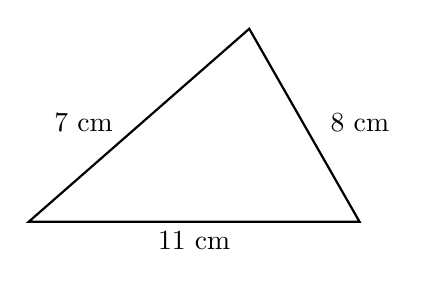
\begin{tikzpicture}[scale=0.7]
  \draw[thick] (0,0) -- (6,0) -- (4,3.5) -- cycle;
  \node[below] at (3,0) {$11$ cm};
  \node[left] at (1.7,1.8) {$7$ cm};
  \node[right] at (5.3,1.8) {$8$ cm};
\end{tikzpicture}
\end{center}
\end{questionText}
\correctAnswer{Yes, it satisfies the inequality and is unique}
\explanation{$7 + 8 = 15 > 11$ \checkmark, $7 + 11 = 18 > 8$ \checkmark, $8 + 11 = 19 > 7$ \checkmark. SSS with valid lengths produces exactly one unique triangle.}
\end{practiceQuestion}

\begin{practiceQuestion}{6-5-q07}{mc}
\begin{questionText}
A triangular prism is sliced with a cut parallel to its triangular base. What is the cross-section?
\end{questionText}
\choiceA{A rectangle}
\choiceB{A triangle congruent to the base}
\choiceC{A smaller triangle}
\choiceD{A trapezoid}
\correctAnswer{B}
\explanation{A cut parallel to the base of a prism always produces a shape congruent (same size and shape) to the base. For a triangular prism, this is a triangle identical to the base.}
\end{practiceQuestion}

\begin{practiceQuestion}{7-3-q03}{mc}
\begin{questionText}
A circle has a diameter of $12$ inches. What is its area? Use $\pi \approx 3.14$.
\end{questionText}
\choiceA{$37.68$ in$^2$}
\choiceB{$113.04$ in$^2$}
\choiceC{$452.16$ in$^2$}
\choiceD{$144$ in$^2$}
\correctAnswer{B}
\explanation{$r = 12 \div 2 = 6$ in. $A = \pi r^2 = 3.14 \times 36 = 113.04$ in$^2$.}
\end{practiceQuestion}

\begin{practiceQuestion}{7-4-q25}{sa}
\begin{questionText}
A trapezoidal garden has parallel sides of $8$ m and $12$ m, and a height of $5$ m. What is its area?
\end{questionText}
\correctAnswer{$50$ m$^2$}
\explanation{$A = \frac{1}{2}(b_1 + b_2) \times h = \frac{1}{2}(8 + 12) \times 5 = \frac{1}{2} \times 20 \times 5 = 50$ m$^2$.}
\end{practiceQuestion}

\begin{practiceQuestion}{7-5-q10}{mc}
\begin{questionText}
A cube has a surface area of $54$ cm$^2$. What is the area of one face?
\end{questionText}
\choiceA{$6$ cm$^2$}
\choiceB{$9$ cm$^2$}
\choiceC{$18$ cm$^2$}
\choiceD{$27$ cm$^2$}
\correctAnswer{B}
\explanation{A cube has $6$ identical faces. Area of one face $= 54 \div 6 = 9$ cm$^2$.}
\end{practiceQuestion}

\begin{practiceQuestion}{7-6-q25}{sa}
\begin{questionText}
Two rectangular prisms have the same base of $5$ cm by $4$ cm. Prism A is $6$ cm tall and Prism B is $9$ cm tall. What is the difference in their volumes?
\end{questionText}
\correctAnswer{$60$ cm$^3$}
\explanation{$V_A = 5 \times 4 \times 6 = 120$ cm$^3$. $V_B = 5 \times 4 \times 9 = 180$ cm$^3$. Difference: $180 - 120 = 60$ cm$^3$.}
\end{practiceQuestion}

\begin{practiceQuestion}{8-1-q07}{mc}
\begin{questionText}
Which of the following is an example of a biased sample?
\end{questionText}
\choiceA{Randomly selecting $50$ names from a hat containing all student names}
\choiceB{Using a random number generator to pick $30$ employees}
\choiceC{Asking every $10$th person who enters a store}
\choiceD{Surveying only members of the basketball team about school sports}
\correctAnswer{D}
\explanation{Basketball players have strong opinions about sports that may not represent the whole school.}
\end{practiceQuestion}

\begin{practiceQuestion}{8-3-q23}{sa}
\begin{questionText}
What does it mean when two box plots have a large gap between them on a number line?
\end{questionText}
\correctAnswer{The two groups have very different values with little or no overlap}
\explanation{A large gap indicates the groups' data ranges do not overlap much, suggesting a clear difference between the populations.}
\end{practiceQuestion}

\begin{practiceQuestion}{8-4-q19}{sa}
\begin{questionText}
Data: $30, 35, 40, 45, 50$. Find the mean and range.
\end{questionText}
\correctAnswer{Mean $= 40$; Range $= 20$}
\explanation{Mean: $\frac{30+35+40+45+50}{5} = \frac{200}{5} = 40$. Range: $50 - 30 = 20$.}
\end{practiceQuestion}

\begin{practiceQuestion}{8-7-q25}{sa}
\begin{questionText}
A double bar graph shows monthly book sales: Store A sold $120$ in March and $150$ in April. Store B sold $100$ in March and $180$ in April. Which store had a greater percent increase from March to April?
\end{questionText}
\correctAnswer{Store B ($80\%$ increase vs.\ $25\%$)}
\explanation{Store A: $\frac{150-120}{120} = \frac{30}{120} = 25\%$. Store B: $\frac{180-100}{100} = \frac{80}{100} = 80\%$. Store B had a greater percent increase.}
\end{practiceQuestion}

\begin{practiceQuestion}{9-4-q28}{gmc}
\begin{questionText}
Look at the two bags below. Which bag represents a uniform probability model for drawing a marble?

\begin{center}
\begin{tikzpicture}[scale=0.65]
  % Bag 1
  \draw[thick,rounded corners=8pt] (-3,-1.5) rectangle (0,1.5);
  \node[above,font=\bfseries] at (-1.5,1.5) {Bag 1};
  \fill[funRed] (-2.3,0.5) circle (0.3);
  \fill[funRed] (-1.5,0.5) circle (0.3);
  \fill[funBlue] (-0.7,0.5) circle (0.3);
  \fill[funBlue] (-2.3,-0.5) circle (0.3);
  \fill[funGreen] (-1.5,-0.5) circle (0.3);
  \fill[funGreen] (-0.7,-0.5) circle (0.3);
  % Bag 2
  \draw[thick,rounded corners=8pt] (1,-1.5) rectangle (4,1.5);
  \node[above,font=\bfseries] at (2.5,1.5) {Bag 2};
  \fill[funRed] (1.7,0.5) circle (0.3);
  \fill[funRed] (2.5,0.5) circle (0.3);
  \fill[funRed] (3.3,0.5) circle (0.3);
  \fill[funRed] (1.7,-0.5) circle (0.3);
  \fill[funBlue] (2.5,-0.5) circle (0.3);
  \fill[funGreen] (3.3,-0.5) circle (0.3);
\end{tikzpicture}
\end{center}
\end{questionText}
\choiceA{Bag 1 only}
\choiceB{Bag 2 only}
\choiceC{Both bags}
\choiceD{Neither bag}
\correctAnswer{A}
\explanation{Bag 1 has $2$ of each color ($2$ red, $2$ blue, $2$ green), so each color is equally likely — uniform. Bag 2 has $4$ red, $1$ blue, $1$ green — non-uniform.}
\end{practiceQuestion}

\begin{practiceQuestion}{9-6-q17}{mc}
\begin{questionText}
Two spinners are spun. Spinner 1 has sections $\{1, 2, 3\}$ and Spinner 2 has sections $\{A, B\}$. What is the probability of getting $2$ and $A$?
\end{questionText}
\choiceA{$\frac{1}{3}$}
\choiceB{$\frac{1}{5}$}
\choiceC{$\frac{1}{6}$}
\choiceD{$\frac{2}{6}$}
\correctAnswer{C}
\explanation{$P(2) = \frac{1}{3}$, $P(A) = \frac{1}{2}$. $P = \frac{1}{3} \times \frac{1}{2} = \frac{1}{6}$.}
\end{practiceQuestion}

\begin{practiceQuestion}{9-7-q19}{sa}
\begin{questionText}
A simulation uses a coin flip ($50\%$ chance) to model whether it rains on a given day. In $30$ trials, rain occurs $16$ times. What is the experimental probability of rain?
\end{questionText}
\correctAnswer{$\frac{16}{30}$}
\explanation{$P = \frac{16}{30} \approx 0.533$.}
\end{practiceQuestion}
